%%%%%%%%%%%%%%%%%%%%%%%%%%%%%%%%%%%%%%%%%%%%%%%%%%%%
% GT-DISS
%
%  Main file to be compiled. Required packages and
%  their options are set in preamble.tex.
%%%%%%%%%%%%%%%%%%%%%%%%%%%%%%%%%%%%%%%%%%%%%%%%%%%%

\documentclass[12pt]{report}

% Load in required packages and settings

% Load in required packages

% For images and plots
\usepackage{graphicx} 
% Set required margins. It's insisted that the left margin be 1.5 in (for printing)
% even for digital coies.
\usepackage[letterpaper, left=1.5in, right=1in, top=1in, bottom=1in]{geometry}
% Allows us to set linespacing conveniently as desired
\usepackage{setspace}  
% Title control and formatting
\usepackage[explicit]{titlesec}  
% Table of contents control and formatting
\usepackage[titles]{tocloft}  
% Set up bibliography formatting
% \usepackage[backend=bibtex, sorting=none, bibstyle=ieee]{biblatex}  
% Load package for appendices
\usepackage[page]{appendix}
% For rotated, landscape images
\usepackage{rotating} 
% For italicized text 
\usepackage[normalem]{ulem}  

% Pretty much indispensible math packages
\usepackage{amsmath}
\usepackage{amsfonts}
\usepackage{amssymb}

% This will allow numbering of subsubsections
\setcounter{secnumdepth}{4}
\setcounter{tocdepth}{4} % Set to 3 to exclude subsubsections from TOC

% Use cite package so we can do superscript citations
\usepackage[superscript]{cite}

% Call it "References" instead of "Bibliography"
\renewcommand\bibname{References}

% Set up footnote style. We'll use symbols to distinguish from superscipt numbers, which
% used for the references. We won't use the asterisk though, because I think it's kinda 
% ugly.
\usepackage[bottom,hang,flushmargin,perpage,symbol*]{footmisc}
\DefineFNsymbols*{lamportnostar}[math]{\dagger\ddagger\S\P\|{\dagger\dagger}{\ddagger\ddagger}}
\setfnsymbol{lamportnostar}
\interfootnotelinepenalty=10000 % Prevent from breaking accross pages

% Use Baskervald Font. This is not one of the recommended fonts, but it is not required
% that we use a font from that list.
\usepackage[lf]{Baskervaldx} % lining figures
\usepackage[bigdelims,vvarbb]{newtxmath} % math italic letters from Nimbus Roman
\usepackage[cal=cm]{mathalfa} % Use mathcal from Computer Modern
\renewcommand*\oldstylenums[1]{\textosf{#1}}
\frenchspacing % Use single spacing after periods

% Set up nomenclature conditions
\usepackage{nomencl}
\makenomenclature
% Set nomenclature title
\renewcommand{\nomname}{List of Symbols}
\renewcommand{\nompreamble}{Effort has been made to use the blow symbols consistently. In the interest of clarity, symbols are occasionally used in isolation for other purposes, in which case their pertinent meaning will be stated.}
% Nomenclature group definitions
\usepackage{ifthen}
\renewcommand{\nomgroup}[1]{%
  \ifthenelse{\equal{#1}{A}}{ {\vskip 6mm} \item[\textbf{Roman Letters}]}{%
  \ifthenelse{\equal{#1}{G}}{ {\vskip 6mm} \item[\textbf{Greek Letters}]}{%
  \ifthenelse{\equal{#1}{M}}{ {\vskip 6mm} \item[\textbf{Mathematical Notations}]}{%
  \ifthenelse{\equal{#1}{S}}{ {\vskip 6mm} \item[\textbf{Subscripts and Superscripts}]}{%
  }}}}%
}

% Load hyperref second to last since it redefines some macros. Make all links black so they
% don't stand out in the PDF
\usepackage[bookmarksnumbered,pdfa]{hyperref}
 \hypersetup{bookmarks=true,
         pdfauthor={Author Name},
         pdftitle={Title of Dissertation},
         pdfsubject={Research Notes},
         pdfkeywords={Keywords},
         colorlinks=true,
         urlcolor=black,
         linkcolor=black,
         citecolor=black}
\usepackage[all]{hypcap}

% Finally, load cleveref, which allows automatic formatting of the references
\usepackage{cleveref}


%%%%%%%%%%%%%%%%%%%%%%
% Start of Document
%%%%%%%%%%%%%%%%%%%%%%

\begin{document}

\doublespacing  %set line spacing

%%%%%%%%%%%%%%%%%%%%%%%%%%%%%%%%%%%%%
% Title Page
%%%%%%%%%%%%%%%%%%%%%%%%%%%%%%%%%%%%%

% This file contains information to be included on the title page

\newcommand{\thesisTitle}{Title of Your Thesis\\on Several Lines if Needed}
\newcommand{\yourName}{Your Name}
\newcommand{\yourSchool}{Mechanical Engineering}
\newcommand{\yourMonth}{January}
\newcommand{\yourYear}{2020}

% --------- The rest is just formatting ---------------

\begin{titlepage}
\begin{center}

\begin{singlespacing}

{\Large\textbf{\textsc{\thesisTitle}}}\\
\vspace{10\baselineskip}
{\footnotesize \textsc{A Dissertation}}\\
{\footnotesize \textsc{Presented to}}\\
{\footnotesize \textsc{The Academic Faculty}}\\
\vspace{2\baselineskip}
{\footnotesize \textsc{By}}\\
\vspace{2\baselineskip}
\large\yourName\\
\vspace{2\baselineskip}
{\footnotesize \textsc{In Partial Fulfillment}}\\
{\footnotesize \textsc{of the Requirements for the Degree}}\\
{\footnotesize \textsc{Doctor of Philosophy in the}}\\
{\footnotesize \textsc{School of \yourSchool}}\\
\vspace{2\baselineskip}
{\large Georgia Institute of Technology}\\
\vspace{\baselineskip}
{\large \yourMonth{} \yourYear{}}
\vfill
\normalsize{\textsc{Copyright \textcopyright{} \yourName{} \yourYear{}}}
\vspace{\baselineskip}

\end{singlespacing}

\end{center}
\end{titlepage}



\currentpdfbookmark{Title Page}{titlePage}  %add PDF bookmark for this page

%%%%%%%%%%%%%%%%%%%%%%%%%%%%%%%%%%%%%
% Approval Page
%%%%%%%%%%%%%%%%%%%%%%%%%%%%%%%%%%%%%

%% Define your committee members. If you have less than 6, simple delete/comment the unused lines

\newcommand{\committeeMemberOne}{Prof.~Olson Johnson, Advisor}
\newcommand{\committeeMemberOneDepartment}{School of Myths}
\newcommand{\committeeMemberOneAffiliation}{Georgia Institute of Technology}

\newcommand{\committeeMemberTwo}{Prof.~Gabby Johnson}
\newcommand{\committeeMemberTwoDepartment}{School of Mechanical Engineering}
\newcommand{\committeeMemberTwoAffiliation}{Georgia Institute of Technology}

\newcommand{\committeeMemberThree}{Prof.~Olson Johnson}
\newcommand{\committeeMemberThreeDepartment}{School of Electrical Engineering}
\newcommand{\committeeMemberThreeAffiliation}{Georgia Institute of Technology}

\newcommand{\committeeMemberFour}{Prof.~Samuel Johnson}
\newcommand{\committeeMemberFourDepartment}{School of Computer Science}
\newcommand{\committeeMemberFourAffiliation}{Georgia Institute of Technology}

\newcommand{\committeeMemberFive}{Prof.~Howard Johnson}
\newcommand{\committeeMemberFiveDepartment}{School of Public Policy}
\newcommand{\committeeMemberFiveAffiliation}{Georgia Institute of Technology}

\newcommand{\committeeMemberSix}{Prof.~Lili von Schtupp}
\newcommand{\committeeMemberSixDepartment}{School of Nuclear Engineering}
\newcommand{\committeeMemberSixAffiliation}{Georgia Institute of Technology}

\newcommand{\approvalDay}{11}
\newcommand{\approvalMonth}{January}
\newcommand{\approvalYear}{2020}

%%%%%%%%%%%%%%%%%%%%%%%%%%%%%%%%%%%%%%%%%%%%%%%%%%%%%%%%%
% Do not edit these lines unless you wish to customize
% the template
%%%%%%%%%%%%%%%%%%%%%%%%%%%%%%%%%%%%%%%%%%%%%%%%%%%%%%%%%


\begin{titlepage}
\begin{singlespacing}
\begin{center}

\textbf{\textsc{\thesisTitle}}\\
\vspace{10\baselineskip}

\end{center}
\vfill

%Define minipages, depending on how many authors there are
\ifdefined\committeeMemberFour

Approved by:
\vspace{2\baselineskip}		% Adjust the number in front of "\baselineskip" for alignment

\begin{minipage}[b]{0.4\textwidth}
	
    \committeeMemberOne\\
    \committeeMemberOneDepartment\\
    \textit{\committeeMemberOneAffiliation}\\
	
    \committeeMemberTwo\\
    \committeeMemberTwoDepartment\\
    \textit{\committeeMemberTwoAffiliation}\\
    
    \committeeMemberThree\\
    \committeeMemberThreeDepartment\\
    \textit{\committeeMemberThreeAffiliation}\\
		
\end{minipage}
\hspace{0.1\textwidth}
\begin{minipage}[b]{0.4\textwidth}
	
	\committeeMemberFour\\
	\committeeMemberFourDepartment\\
	\textit{\committeeMemberFourAffiliation}\\
	
	\ifdefined\committeeMemberSix

	  \committeeMemberFive\\
	  \committeeMemberFiveDepartment\\
	  \textit{\committeeMemberFiveAffiliation}\\
	
	  \committeeMemberSix\\
	  \committeeMemberSixDepartment\\
	  \textit{\committeeMemberSixAffiliation}\\
	
	\else
	
	  \committeeMemberFive\\
	  \committeeMemberFiveDepartment\\
	  \textit{\committeeMemberFiveAffiliation}\\
	
	\fi
	
\end{minipage}\\

% Add approval date
\begin{minipage}[b]{0.4\textwidth}

  ~% Empty minipage for alignment	

\end{minipage}
\hspace{0.1\textwidth}
\begin{minipage}[b]{0.4\textwidth}
    Date Approved: \approvalMonth{} \approvalDay, \approvalYear
    \vspace{5\baselineskip}		%adjust the number in front of "\baselineskip" for alignment	
\end{minipage}\\

\else

\hspace{0.6\textwidth}
\begin{minipage}[b]{0.4\textwidth}
	
	Approved by:
	\vspace{2\baselineskip}		%adjust the number in front of "\baselineskip" for alignment
	
	\committeeMemberOne\\
	\committeeMemberOneDepartment\\
	\textit{\committeeMemberOneAffiliation}\\
	
	\committeeMemberTwo\\
	\committeeMemberTwoDepartment\\
	\textit{\committeeMemberTwoAffiliation}\\
	
	\committeeMemberThree\\
	\committeeMemberThreeDepartment\\
	\textit{\committeeMemberThreeAffiliation}\\
	
	\vspace{2\baselineskip}		%adjust the number in front of "\baselineskip" for alignment
	
	Date Approved: \approvalMonth{} \approvalDay, \approvalYear
	\vspace{\baselineskip}		%adjust the number in front of "\baselineskip" for alignment
	
\end{minipage}

\fi





\end{singlespacing}
\end{titlepage}


%%%%%%%%%%%%%%%%%%%%%%%%%%%%%%%%%%%%%
% Epigraph
%%%%%%%%%%%%%%%%%%%%%%%%%%%%%%%%%%%%%

% Define your quote and author for the epigraph here

\newcommand{\yourQuote}{A great quote to start the thesis}
\newcommand{\yourAuthor}{George P. Burdell}

%%%%%%%%%%%%%%%%%%%%%%%%%%%%%%%%%%%%%%%%%%%%%%%%%%%%%%%%%
% Do not edit these lines unless you wish to customize
% the template
%%%%%%%%%%%%%%%%%%%%%%%%%%%%%%%%%%%%%%%%%%%%%%%%%%%%%%%%%

\begin{titlepage}
\begin{center}

\vspace*{\fill}
\yourQuote\\
\textit{\yourAuthor}
\vspace*{\fill}

\end{center}
\end{titlepage}



%%%%%%%%%%%%%%%%%%%%%%%%%%%%%%%%%%%%%
% Dedication
%%%%%%%%%%%%%%%%%%%%%%%%%%%%%%%%%%%%%

% Define your dedication statement here

\newcommand{\yourDedication}{A great dedication goes here.}

%%%%%%%%%%%%%%%%%%%%%%%%%%%%%%%%%%%%%%%%%%%%%%%%%%%%%%%%%
% Do not edit these lines unless you wish to customize
% the template
%%%%%%%%%%%%%%%%%%%%%%%%%%%%%%%%%%%%%%%%%%%%%%%%%%%%%%%%%

\begin{titlepage}
\begin{center}

\vspace*{\fill}
\yourDedication\\
\vspace*{\fill}

\end{center}
\end{titlepage}


%%%%%%%%%%%%%%%%%%%%%%%%%%%%%%%%%%%%%
% Acknowledgments
%%%%%%%%%%%%%%%%%%%%%%%%%%%%%%%%%%%%%

\pagenumbering{roman}
\addcontentsline{toc}{chapter}{Acknowledgments}

% Set the page number appropriately based on the number of intro pages
\setcounter{page}{5} 
\clearpage
\begin{centering}
\textbf{ \Large Acknowledgements}\\
\vspace{\baselineskip}
\end{centering}

%Insert your dedication text here
Lorem ipsum dolor sit amet, consectetur adipiscing elit, sed do eiusmod tempor incididunt ut labore et dolore magna aliqua. Ut enim ad minim veniam, quis nostrud exercitation ullamco laboris nisi ut aliquip ex ea commodo consequat. Duis aute irure dolor in reprehenderit in voluptate velit esse cillum dolore eu fugiat nulla pariatur. Excepteur sint occaecat cupidatat non proident, sunt in culpa qui officia deserunt mollit anim id est laborum.

\clearpage
%\pagenumbering{gobble}  %remove page number on summary page


%\addtocontents{toc}{\cftpagenumbersoff{chapter}} 

%\currentpdfbookmark{Acknowledgments}{acknowledgments}
%\addtocontents{toc}{\cftpagenumberson{chapter}} 

%%%%%%%%%%%%%%%%%%%%%%%%%%%%%%%%%%%%%
% Table of Contents
%%%%%%%%%%%%%%%%%%%%%%%%%%%%%%%%%%%%%

% Format for Table of Contents
\renewcommand{\cftchapdotsep}{\cftdotsep}  %add dot separators
\renewcommand{\cftchapfont}{\bfseries}  %set title font weight
\renewcommand{\cftchappagefont}{}  %set page number font weight
\renewcommand{\cftchappresnum}{Chapter }
\renewcommand{\cftchapaftersnum}{:~~}
\renewcommand{\cftchapnumwidth}{5em}
\renewcommand{\cftchapafterpnum}{\vskip\baselineskip} %set correct spacing for entries in single space environment
\renewcommand{\cftsecafterpnum}{\vskip\baselineskip}  %set correct spacing for entries in single space environment
\renewcommand{\cftsubsecafterpnum}{\vskip\baselineskip} %set correct spacing for entries in single space environment
\renewcommand{\cftsubsubsecafterpnum}{\vskip\baselineskip} %set correct spacing for entries in single space environment

%format title font size and position (this also applys to list of figures and list of tables)
\titleformat{\chapter}[display]
{\Large\bfseries\filcenter}{\chaptertitlename\ \thechapter}{0pt}{#1}

\renewcommand\contentsname{Table of Contents}

% Print table of contents
{\singlespacing
\tableofcontents
}

\currentpdfbookmark{Table of Contents}{TOC}

\clearpage

%%%%%%%%%%%%%%%%%%%%%%%%%%%%%%%%%%%%%
% List of figures and tables
%%%%%%%%%%%%%%%%%%%%%%%%%%%%%%%%%%%%%

\addcontentsline{toc}{chapter}{List of Tables}
\begin{singlespace}
	\setlength\cftbeforetabskip{\baselineskip}  %manually set spacing between entries
	\listoftables
\end{singlespace}

\clearpage

\addcontentsline{toc}{chapter}{List of Figures}
\begin{singlespace}
\setlength\cftbeforefigskip{\baselineskip}  %manually set spacing between entries
\listoffigures
\end{singlespace}

\clearpage

%%%%%%%%%%%%%%%%%%%%%%%%%%%%%%%%%%%%%%%%%%%%%%%%%%%%%%%%%%%%%%%%%
% This is the Summary (abstract should be separate document)
%%%%%%%%%%%%%%%%%%%%%%%%%%%%%%%%%%%%%%%%%%%%%%%%%%%%%%%%%%%%%%%%%

\clearpage
\begin{centering}
\textbf{SUMMARY}\\
\vspace{\baselineskip}
\end{centering}

Lorem ipsum dolor sit amet, consectetur adipiscing elit, sed do eiusmod tempor incididunt ut labore et dolore magna aliqua. Ut enim ad minim veniam, quis nostrud exercitation ullamco laboris nisi ut aliquip ex ea commodo consequat. Duis aute irure dolor in reprehenderit in voluptate velit esse cillum dolore eu fugiat nulla pariatur. Excepteur sint occaecat cupidatat non proident, sunt in culpa qui officia deserunt mollit anim id est laborum.

%\pagenumbering{gobble}  %remove page number on summary page

%%%%%%%%%%%%%%%%%%%%%%%%%%%%
%
% Chapters
%
%%%%%%%%%%%%%%%%%%%%%%%%%%%%

%%%%%%%%%%%%%%%%%%%%%%
% formatting
%%%%%%%%%%%%%%%%%%%%%%

% resume page numbering for rest of document
\clearpage
\pagenumbering{arabic}
\setcounter{page}{1} % set the page number appropriately

% From the manual: "Chapters are customarily divided into subsections with subheadings
% that have slightlydiffering font styles and are designated first, second, and third-
% level. The first-level subdivision should have greater attention value than the lower
% levels. Centered headings have more attention value than headings beginning at the
% left margin, and italic, underlining, or bold-face type has more attention value than
% plain text. Attention value is also enhanced by leaving some blank space above and
% below". The "customarily" languate differs from language elsewhere in the document
% indicates compulsion (e.g., "must", "Leave three blank lines", etc.). Therefore I 
% interpret the section formatting as suggested, and ignore the suggestion, as I think
% changing fonts, weights, and styles is distracting. The new line, coupled with the 
% section number (e.g., 2.1.4) clearly indicates its importance.

% Format Chapter headings
\titleformat{\chapter}[display]% 
{\filcenter\bfseries\Large}% Chapter Title Font
{Chapter~\thechapter}% Label
{-1mm} % Separation
{#1}
\titlespacing*{\chapter}
  {0pt}{0pt}{30pt}	%controls vertical margins on title
  
% Adjust section title formatting
\titleformat{\section}{\large\bfseries}{\thesection\hspace{2mm}}{0pt}{#1}

% Adjust subsection title formatting
\titleformat{\subsection}{\bfseries}{\thesubsection\hspace{2.5mm}}{0pt}{#1}

% Adjust subsubsection title formatting
\titleformat{\subsubsection}{\bfseries}{\thesubsubsection\hspace{3mm}}{0pt}{#1}

%%%%%%%%%%%%%%%%
% Chapter 1
%%%%%%%%%%%%%%%%

\chapter{Introduction and Background}

\section{About this Template}
This template is an adaptation \texttt{gatechthesis\_latex} template (17 January 2017 update) and \texttt{ut-diss-2}. 
I've made some (mostly) aesthetic changes, but I believe it should conform to the requirements liseted in the Georgia Tech ``Graduate Thesis/Dissertation Guidelines \& Procedures'' (April 2015 Update).
It is by no means an official template, though. 
So as stated in the license file, you can use, change, distribute, sell it however you'd like, provided
\begin{enumerate}
  \item You include the copyright notice in the license file; and
  \item You hold none of the authors liable for any results of such use.
\end{enumerate}

\section{Basic Elements}
This section talks about common components (figures, tables, and equations), and how they're included in \LaTeX{} documents.
Much better and more complete resources are available elsewhere, but hopefully this enough to get started.

\subsection{Figures}
Figures are included with the \texttt{figure} environment.
They are floats, which means that they will appear wherever \LaTeX{} thinks is best based on the surrounding text.
You can tinker with this positioning, but the details are out of scope.
A quick example will give most of the salient details. 
The following code will give the results in \cref{fig:IntensityVsWavelength}.
\begin{minipage}{0.75\textwidth}
\footnotesize
  \vspace{2mm}
  \begin{verbatim}
\begin{figure}
  \centering
  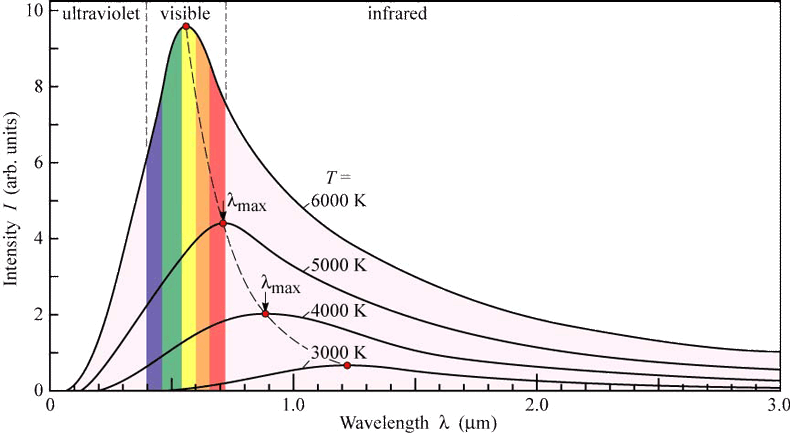
\includegraphics[width=0.75\linewidth]{figures/exampleFigure.png}
  \caption[Short Caption]{This is a long caption. It's too long  
         for the table of contents, so we specify a short caption 
         in the brackets.}
  \label{fig:IntensityVsWavelength}
\end{figure}
  \end{verbatim}
  \vspace{2mm}
\end{minipage}

Note the use of a short caption in brackets in the \texttt{\textbackslash caption} command.
This lets us have a long explanatory caption, without keeping our List of Tables compact (compare the caption of \cref{fig:IntensityVsWavelength}) with how it's listed on \cpageref{sec:ListOfTables}.

\begin{figure}
  \centering
  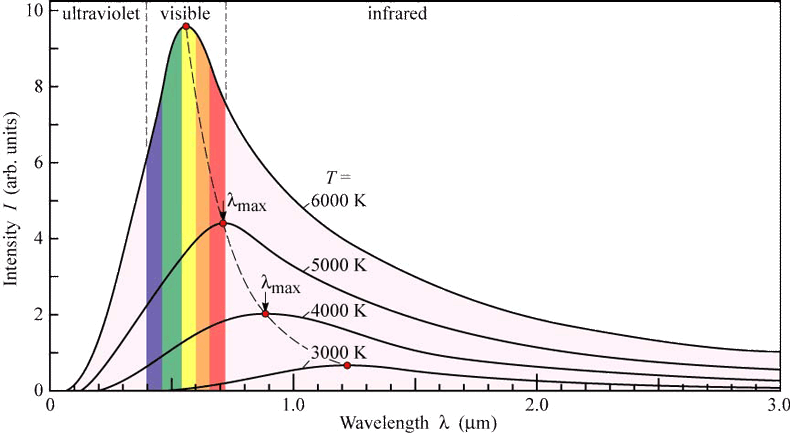
\includegraphics[width=0.75\linewidth]{figures/exampleFigure.png}
  \caption[Short Caption]{This is a long caption. It's too long  
         for the table of contents, so we specify a short caption 
         in the brackets.}
  \label{fig:IntensityVsWavelength}
\end{figure}

\subsection{Tables}


\subsection{Equations}
I recommend using the \texttt{align} environment exclusively for equations. 
It's virtually identical to \texttt{equation}, but allows you to have multiple lines and specify where you want them to---well---\emph{align} with each other.
Compare the following\\
\begin{minipage}[t]{0.48\textwidth}
\small
\begin{verbatim}
\begin{equation}
  a^{2} + b^{2} = c^{2}
\end{equation}
\end{verbatim}
\begin{equation}
  a^{2} + b^{2} = c^{2}
\end{equation}
\end{minipage}
~
\begin{minipage}[t]{0.48\textwidth}
\small
\begin{verbatim}
\begin{align}
  a^{2} + b^{2} = c^{2}
\end{align}
\end{verbatim}
\begin{align}
  a^{2} + b^{2} = c^{2}
\end{align}
\end{minipage}


\section{Cross-Referencing}
One of the chief advantages of \LaTeX{} is how easy it makes cross-references.
Note that we often want to refer to a figure or equation.
Sure, we could number them by hand, but it we insert or delete 


Items are referenced using \texttt{cleveref} and \texttt{hyperref} packages. For example, here's an equation
\begin{align}
   i\hbar\frac{\partial}{\partial t}\Psi &= \left[ \frac{-\hbar^{2}}{2m}\nabla^{2} + V\right]\Psi\,.
  \label{eqn:SchrodingerEquation}
\end{align}
\Cref{eqn:SchrodingerEquation} should be referenced as so.

Lorem ipsum dolor sit amet, consectetur adipiscing elit, sed do eiusmod tempor incididunt ut labore et dolore magna aliqua. Ut enim ad minim veniam, quis nostrud exercitation ullamco laboris nisi ut aliquip ex ea commodo consequat \cite{ref1}. Duis aute irure dolor in reprehenderit in voluptate velit esse cillum dolore eu fugiat nulla pariatur \cite{ref2}. Excepteur sint occaecat cupidatat non proident, sunt in culpa qui officia deserunt mollit anim id est laborum.

Lorem ipsum dolor sit amet, consectetur adipiscing elit, sed do eiusmod tempor incididunt ut labore et dolore magna aliqua. Ut enim ad minim veniam, quis nostrud exercitation ullamco laboris nisi ut aliquip ex ea commodo consequat \cite{ref1}. Duis aute irure dolor in reprehenderit in voluptate velit esse cillum dolore eu fugiat nulla pariatur \cite{ref2}. Excepteur sint occaecat cupidatat non proident, sunt in culpa qui officia deserunt mollit anim id est laborum.

Lorem ipsum dolor sit amet, consectetur adipiscing elit, sed do eiusmod tempor incididunt ut labore et dolore magna aliqua. Ut enim ad minim veniam, quis nostrud exercitation ullamco laboris nisi ut aliquip ex ea commodo consequat \cite{ref1}. Duis aute irure dolor in reprehenderit in voluptate velit esse cillum dolore eu fugiat nulla pariatur \cite{ref2}. Excepteur sint occaecat cupidatat non proident, sunt in culpa qui officia deserunt mollit anim id est laborum.

Lorem ipsum dolor sit amet, consectetur adipiscing elit, sed do eiusmod tempor incididunt ut labore et dolore magna aliqua. Ut enim ad minim veniam, quis nostrud exercitation ullamco laboris nisi ut aliquip ex ea commodo consequat \cite{ref1}. Duis aute irure dolor in reprehenderit in voluptate velit esse cillum dolore eu fugiat nulla pariatur \cite{ref2}. Excepteur sint occaecat cupidatat non proident, sunt in culpa qui officia deserunt mollit anim id est laborum.

Lorem ipsum dolor sit amet, consectetur adipiscing elit, sed do eiusmod tempor incididunt ut labore et dolore magna aliqua. Ut enim ad minim veniam, quis nostrud exercitation ullamco laboris nisi ut aliquip ex ea commodo consequat \cite{ref1}. Duis aute irure dolor in reprehenderit in voluptate velit esse cillum dolore eu fugiat nulla pariatur \cite{ref2}. Excepteur sint occaecat cupidatat non proident, sunt in culpa qui officia deserunt mollit anim id est laborum.

% This is a table

\begin{table}
\caption{This is an example Table.}
\begin{center}
\begin{tabular}{ccc}
$x$ & $f(x)$ & $g(x)$ \\
\hline
1 & 6 & 4  \\
2 & 6 & 3  \\
3 & 6 & 2  \\
4 & 6 & 2  \\
\label{tab:ValuesOfFunctions}
\end{tabular}
\end{center}
\end{table}


%%%%%%%%%%%%%%%%
% Chapter 2
%%%%%%%%%%%%%%%%

\chapter{Technical Approach}
Lorem ipsum dolor sit amet, consectetur adipiscing elit, sed do eiusmod tempor incididunt ut labore et dolore magna aliqua. Ut enim ad minim veniam, quis nostrud exercitation ullamco laboris nisi ut aliquip ex ea commodo consequat. Duis aute irure dolor in reprehenderit in voluptate velit esse cillum dolore eu fugiat nulla pariatur. Excepteur sint occaecat cupidatat non proident, sunt in culpa qui officia deserunt mollit anim id est laborum.

\section{Section}

This is a section in Chapter 2.

\subsection{Example Subsection}

This is a subsection in Chapter 2.

\subsubsection{Example Subsubsection}

This is a subsubsection in Chapter 2.

% This is a figure in landscape orientation
\begin{sidewaysfigure}
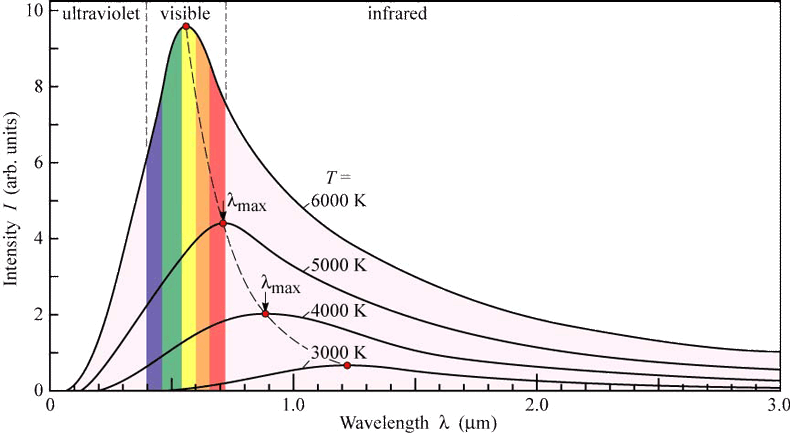
\includegraphics[width=\textwidth]{figures/exampleFigure.png}
\caption{This is another example Figure, rotated to landscape orientation.}
\label{LandscapeFigure}
\end{sidewaysfigure}


%%%%%%%%%%%%%%%%
% Chapter 3
%%%%%%%%%%%%%%%%

\chapter{Results}
Lorem ipsum dolor sit amet, consectetur adipiscing elit, sed do eiusmod tempor incididunt ut labore et dolore magna aliqua. Ut enim ad minim veniam, quis nostrud exercitation ullamco laboris nisi ut aliquip ex ea commodo consequat. Duis aute irure dolor in reprehenderit in voluptate velit esse cillum dolore eu fugiat nulla pariatur. Excepteur sint occaecat cupidatat non proident, sunt in culpa qui officia deserunt mollit anim id est laborum.


%%%%%%%%%%%%%%%%
% Chapter 4
%%%%%%%%%%%%%%%%

\chapter{Discussion}
Lorem ipsum dolor sit amet, consectetur adipiscing elit, sed do eiusmod tempor incididunt ut labore et dolore magna aliqua. Ut enim ad minim veniam, quis nostrud exercitation ullamco laboris nisi ut aliquip ex ea commodo consequat. Duis aute irure dolor in reprehenderit in voluptate velit esse cillum dolore eu fugiat nulla pariatur. Excepteur sint occaecat cupidatat non proident, sunt in culpa qui officia deserunt mollit anim id est laborum..


%%%%%%%%%%%%%%%%
% Chapter 5
%%%%%%%%%%%%%%%%

\chapter{Conclusion}
Lorem ipsum dolor sit amet, consectetur adipiscing elit, sed do eiusmod tempor incididunt ut labore et dolore magna aliqua. Ut enim ad minim veniam, quis nostrud exercitation ullamco laboris nisi ut aliquip ex ea commodo consequat. Duis aute irure dolor in reprehenderit in voluptate velit esse cillum dolore eu fugiat nulla pariatur. Excepteur sint occaecat cupidatat non proident, sunt in culpa qui officia deserunt mollit anim id est laborum.


%%%%%%%%%%%%%%%%
% Appendices
%%%%%%%%%%%%%%%%

\begin{appendices}

%Some Table of Contents entry formatting
\addtocontents{toc}{\protect\renewcommand{\protect\cftchappresnum}{\appendixname\space}}
\addtocontents{toc}{\protect\renewcommand{\protect\cftchapnumwidth}{6em}}

%Begin individual appendices, separated as chapters

\chapter{Experimental Equipment}
Lorem ipsum dolor sit amet, consectetur adipiscing elit, sed do eiusmod tempor incididunt ut labore et dolore magna aliqua. Ut enim ad minim veniam, quis nostrud exercitation ullamco laboris nisi ut aliquip ex ea commodo consequat. Duis aute irure dolor in reprehenderit in voluptate velit esse cillum dolore eu fugiat nulla pariatur. Excepteur sint occaecat cupidatat non proident, sunt in culpa qui officia deserunt mollit anim id est laborum.

\chapter{Data Processing}
Lorem ipsum dolor sit amet, consectetur adipiscing elit, sed do eiusmod tempor incididunt ut labore et dolore magna aliqua. Ut enim ad minim veniam, quis nostrud exercitation ullamco laboris nisi ut aliquip ex ea commodo consequat. Duis aute irure dolor in reprehenderit in voluptate velit esse cillum dolore eu fugiat nulla pariatur. Excepteur sint occaecat cupidatat non proident, sunt in culpa qui officia deserunt mollit anim id est laborum.

\end{appendices}

%%%%%%%%%%%%%%%%
% References
%%%%%%%%%%%%%%%%

{ \singlespacing				   
\bibliographystyle{bibliography/jasanum} 
\bibliography{bibliography/demoReferences}    
}

%%%%%%%%%%%%%%%%
% Vita 
% Only for PhD students
% Masters students remove this line
%%%%%%%%%%%%%%%%
\chapter*{Vita}
\addcontentsline{toc}{chapter}{Vita}  %add Vita section to Table of Contents
Vita may be provided by doctoral students only. The length of the vita is preferably one page. It may include the place of birth and should be written in third person. This vita is similar to the author biography found on book jackets.


\end{document}
